\subsection{Versão 2 - Alteração para Lei Nº 13.409 de 2016 }
\label{versao2}
 Em função da criação da Lei nº 13.409, que altera a lei original nº 12.711, foi feita uma re-estruturação do código para inclusão de novas categorias de cotas para \gls{PCD}, mantendo as outras categorias já existentes. Os trechos de lei afetados foram:
\begin{citacao}
Art. 3º Em cada instituição federal de ensino superior, as vagas de que trata o art. 1º desta Lei serão preenchidas, por curso e turno, por autodeclarados pretos, pardos e indígenas e por pessoas com deficiência, nos termos da legislação, em proporção ao total de vagas no mínimo igual à proporção respectiva de pretos, pardos, indígenas e pessoas com deficiência na população da unidade da Federação onde está instalada a instituição, segundo o último censo da Fundação Instituto Brasileiro de Geografia e Estatística - IBGE.

Art. 5º Em cada instituição federal de ensino técnico de nível médio, as vagas de que trata o art. 4º desta Lei serão preenchidas, por curso e turno, por autodeclarados pretos, pardos e indígenas e por pessoas com deficiência, nos termos da legislação, em proporção ao total de vagas no mínimo igual à proporção respectiva de pretos, pardos, indígenas e pessoas com deficiência na população da unidade da Federação onde está instalada a instituição, segundo o último censo do IBGE \cite{leicotas2}.
\end{citacao}

A equipe de desenvolvimento original do sistema já não estava mais presente no setor e a falta de experiência nas regras de cotas por parte da equipe atual, acabou por dificultar e atrasar o processo de entendimento do código fonte para aplicação das mudanças no sistema,  demandando também a alocação de mais desenvolvedores para divisão do trabalho de codificação dos novos tipos de cota.

Após a análise dos novos trechos de lei foi especificada uma nova versão do algoritmo de classificação, desenvolvida por meio de interpretação da área demandante e dos analistas de sistemas da \gls{DTIC}, gerando uma nova implementação contendo 7 (sete) tipos de categorias de cotas possíveis, conforme Tabela \ref{tabela_cotas_v2}:

\begin{table}[!ht]
\caption{Categorias de cotas na versão 2}
\label{tabela_cotas_v2}
\resizebox{\textwidth}{!}{
\begin{tabular}{|l|l|l|}
\hline
\multirow{6}{*}{\textbf{\begin{tabular}[c]{@{}l@{}}Cotas (EP)\\ mínimo 50\% das vagas\end{tabular}}} & \multirow{3}{*}{\begin{tabular}[c]{@{}l@{}}Renda Inferior do que 1,5 S.M.\\ \\ RI 50\% das cotas   \\ \\
\end{tabular}} & PPI – Pretos Pardos e Índios*           \\ \cline{3-3} 
                                                                                                     &                                                                                                                         & PCD – Pessoas com Deficiência*          \\ \cline{3-3} 
                                                                                                     &                                                                                                                         & NPPID – Não incluídos nos casos acima** \\ \cline{2-3} 
                                                                                                     & \multirow{3}{*}{\begin{tabular}[c]{@{}l@{}}Renda Superior a 1,5 S.M.\\ \\ RS 50\% das cotas  \\ \\ \end{tabular}}       & PPI – Pretos Pardos e Índios*           \\ \cline{3-3} 
                                                                                                     &                                                                                                                         & PCD – Pessoas com Deficiência*          \\ \cline{3-3} 
                                                                                                     &                                                                                                                         & NPPID – Não incluídos nos casos acima** \\ \hline
\multicolumn{3}{|l|}{\textbf{\begin{tabular}[c]{@{}l@{}}Classificação Geral (CLAG)\\ \\ vagas restantes além das cotas\\ \\ máximo 50\% das vagas\end{tabular}}}                                                                                                         \\ \hline
\end{tabular}}
\centering
\par\medskip\textbf{Fonte:} Elaborada pelo autor (2019). \par\medskip
\end{table}

\newpage
O desenvolvimento durou cerca de 3 (três) meses, com 2 (dois) desenvolvedores dedicados, os quais trabalharam em todos os arquivos descritos na primeira versão, assim como as telas envolvidas para atender a este novo entendimento e disponibilizar o Código Fonte \ref{lst:algoritmov2}:

\lstinputlisting[language=PHP, 
caption= Segunda versão do algoritmo
,label=lst:algoritmov2]{chapters/trechos_codigo/algoritmov2.m}

Esse algorítimo substitui o corpo da função \texttt{calcula\_vagasAcoesAfirmativas}, detalhada no Código Fonte \ref{lst:quadrovagas}. Como resultado da geração do quadro de vagas na versão 2, a Figura \ref{fig:cenario2} demonstra o novo cenário para um curso com 40 vagas.

\begin{figure}[ht!]
\centering

\caption{\textmd{Cenário de distribuição versão 2}}
\label{fig:cenario2}
\fcolorbox{gray}{white}{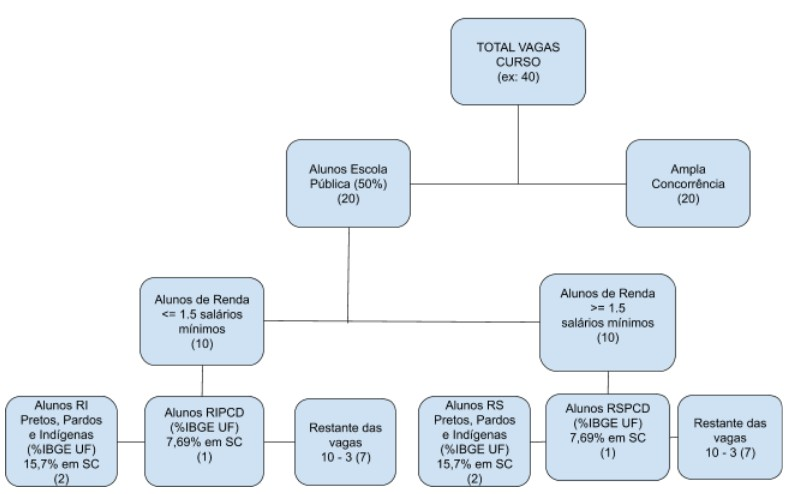
\includegraphics[width=\textwidth]{chapters/sistemaingresso_versoes/cenarios/cenario2.jpg}}

\par\medskip\textbf{Fonte:} Elaborada pelo autor (2019). \par\medskip
\end{figure}



É importante ressaltar que o entendimento de lei repassado pela área demandante se deu sem definição formal do \gls{MEC}, a análise foi procedida por meio de interpretação própria do \gls{IFSC}, e também não havia sido definido como priorizar a sobra de vagas entre cotas, uma vez que a portaria nº 18/2012/MEC  demorou a ser atualizada. Mesmo sem definição clara, o \gls{IFSC} aplicou em seus processos a nova regra de cotas, incluindo reserva para \gls{PCD}.

Após alguns meses em funcionamento desta versão, o \gls{MEC} em resposta oficial, em função das dúvidas das instituições, acabou por modificar novamente a distribuição de vagas, que agora seria em 9 (nove) categorias de cotas diferentes, e também foram atualizadas as regras de priorização em caso de sobra de vaga. Nesse sentido, na Seção \ref{versao3} são apresentados os dados de desenvolvimento da versão atualmente utilizada nos processos seletivos.